\newpage
\chapter*{Anexo I: Ejemplo de procesamiento de impulsos}
\label{ch:anexo_i}
\addcontentsline{toc}{chapter}{Anexo I: Ejemplo de procesamiento de impulsos}
\vspace{3\baselineskip}

A continuación se ilustra de manera secuencial el procesamiento digital del impulso mediante el motor de cálculo, desarrollado de acuerdo con la norma IEC 60060~\cite{iec60060_1} y detallado en la sección \ref{subsec:motor_calculo}.

\section*{Ejemplo de impulso LI}
\label{sec:ejemplo_impulso_li}
\addcontentsline{toc}{section}{Ejemplo de impulso LI}
\vspace{3\baselineskip}

El impulso tipo rayo pleno (LI) analizado en esta sección proviene de la base de datos del Laboratorio de Alta Tensión (LAT). Esta señal fue adquirida mediante el osciloscopio Owon PDS7102T durante un ensayo real y, posteriormente, se acondicionó sus datos para ser procesada por el motor de cálculo. Por lo tanto, este ejemplo refleja con precisión el escenario de aplicación práctica para el cual fue diseñado el software.

En la figura \ref{fig:curva_original} se presenta la señal discreta bruta $U_\text{e}[n]$ tal como fue adquirida por el instrumento, evidenciando la presencia de ruido electromagnético de alta frecuencia y de una componente de tensión continua (\emph{offset}) previa al disparo.

\vspace{3\baselineskip}
\begin{figure}[H]
    \centering
    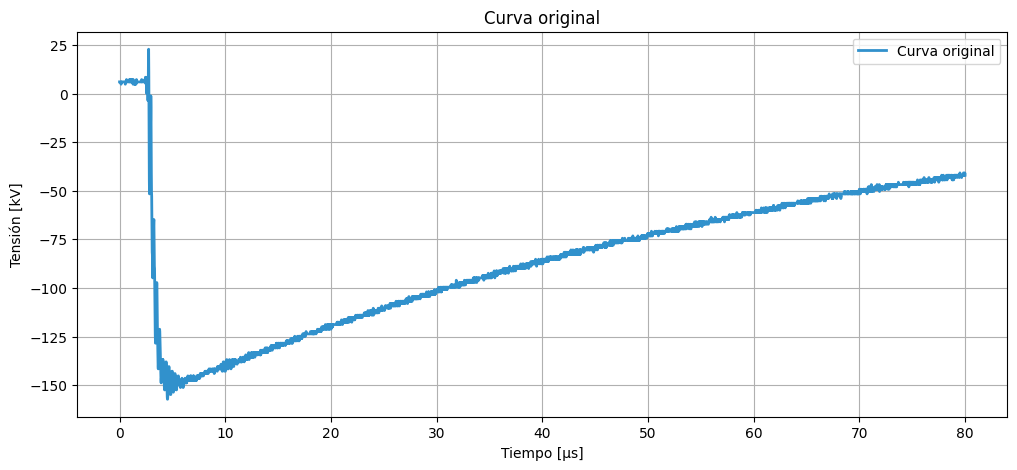
\includegraphics[width=\textwidth]{img/analisis_secuencial/LAT/0_curva_original.png}
    \caption{Adquisición de datos. Fuente: Propia.}
    \label{fig:curva_original}
\end{figure}
\vspace{3\baselineskip}

La figura \ref{fig:curva_offset} muestra la señal resultante tras la sustracción del nivel de continua $V_\text{offset}$, el cual se determinó con las muestras previas al instante de disparo.

\vspace{3\baselineskip}
\begin{figure}[H]
    \centering
    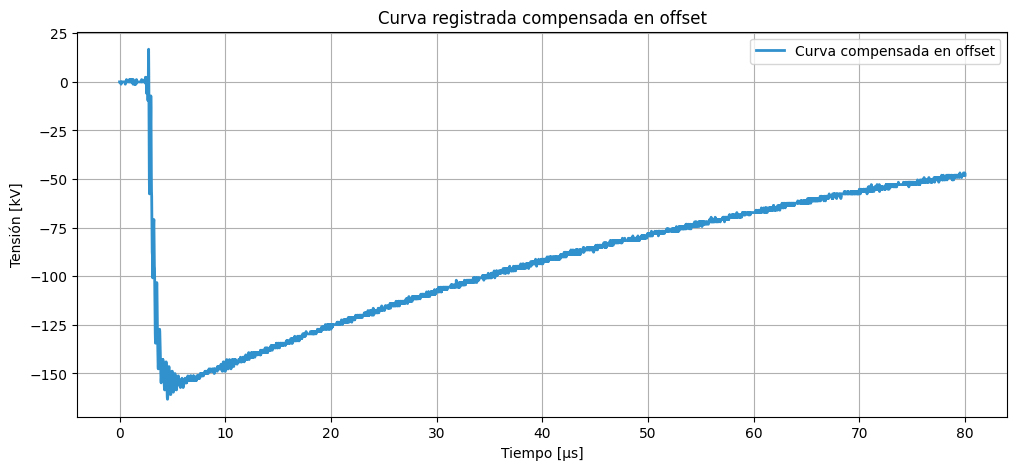
\includegraphics[width=\textwidth]{img/analisis_secuencial/LAT/1_offset_removido.png}
    \caption{Acondicionamiento de continua. Fuente: Propia.}
    \label{fig:curva_offset}
\end{figure}
\vspace{3\baselineskip}

En la figura \ref{fig:curva_positiva} se observa la curva con su polaridad normalizada hacia el semiplano positivo. Este paso estandariza y facilita los cálculos algorítmicos posteriores, independientemente de la polaridad original del impulso.

\vspace{3\baselineskip}
\begin{figure}[H]
    \centering
    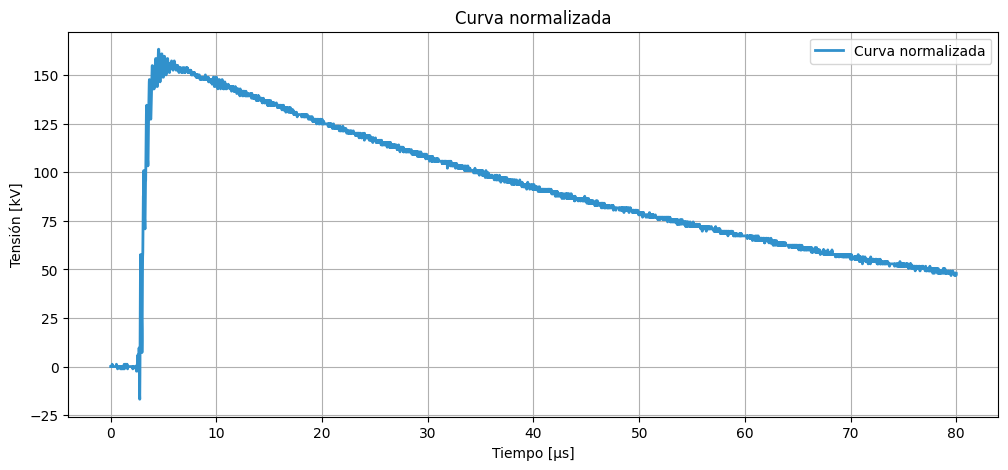
\includegraphics[width=\textwidth]{img/analisis_secuencial/LAT/2_curva_normalizada.png}
    \caption{Normalización de polaridad. Fuente: Propia.}
    \label{fig:curva_positiva}
\end{figure}
\vspace{3\baselineskip}

La figura \ref{fig:curva_recortada} resalta en color rojo la ventana de datos útil (comprendida entre el \qty{20}{\percent} del frente y el \qty{40}{\percent} de la cola). Esta porción es la que se somete al proceso de regresión no lineal mediante el algoritmo de Levenberg-Marquardt~\cite{Chapra2015}.

\vspace{3\baselineskip}
\begin{figure}[H]
    \centering
    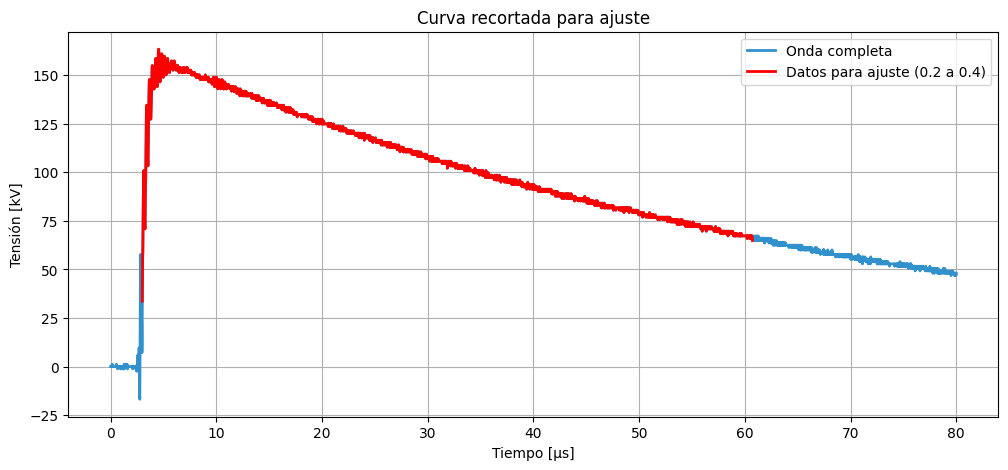
\includegraphics[width=\textwidth]{img/analisis_secuencial/LAT/3_curva_recortada.png}
    \caption{Segmentación de datos. Fuente: Propia.}
    \label{fig:curva_recortada}
\end{figure}
\vspace{3\baselineskip}

Una vez finalizado el ajuste paramétrico, se sintetiza la curva base $U_\text{b}[n]$ empleando la función doble exponencial (ecuación \ref{eq:doble_exponencial}), como se ilustra en la figura \ref{fig:curva_base}. Para evidenciar la diferencia morfológica, se superpuso la curva base idealizada (en trazo rojo) sobre la señal registrada compensada en \emph{offset} (en trazo fino celeste).

\vspace{3\baselineskip}
\begin{figure}[H]
    \centering
    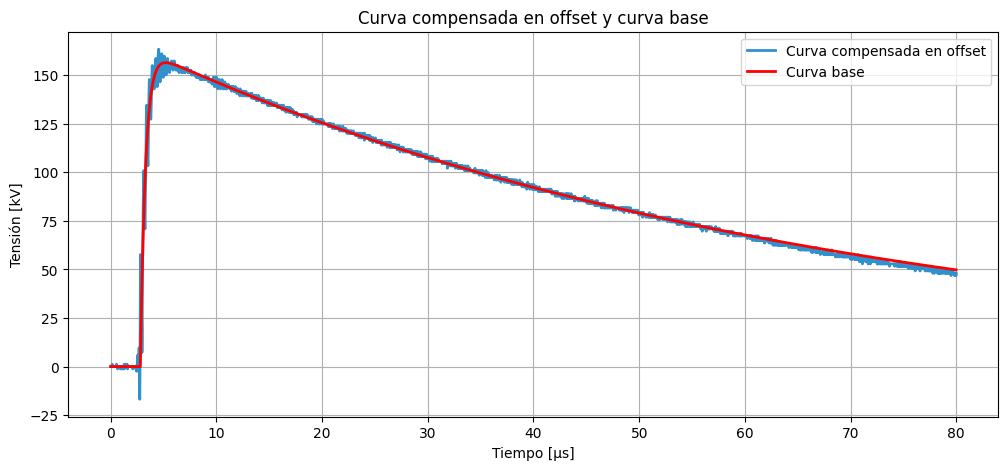
\includegraphics[width=\textwidth]{img/analisis_secuencial/LAT/4_curva_base.png}
    \caption{Sintetización de la curva base. Fuente: Propia.}
    \label{fig:curva_base}
\end{figure}
\vspace{3\baselineskip}

La figura \ref{fig:curva_residual} presenta la curva residual $R[n]$, obtenida mediante la resta algebraica punto a punto entre la señal compensada y la curva base, logrando así aislar las oscilaciones y el ruido superpuesto.

\vspace{3\baselineskip}
\begin{figure}[H]
    \centering
    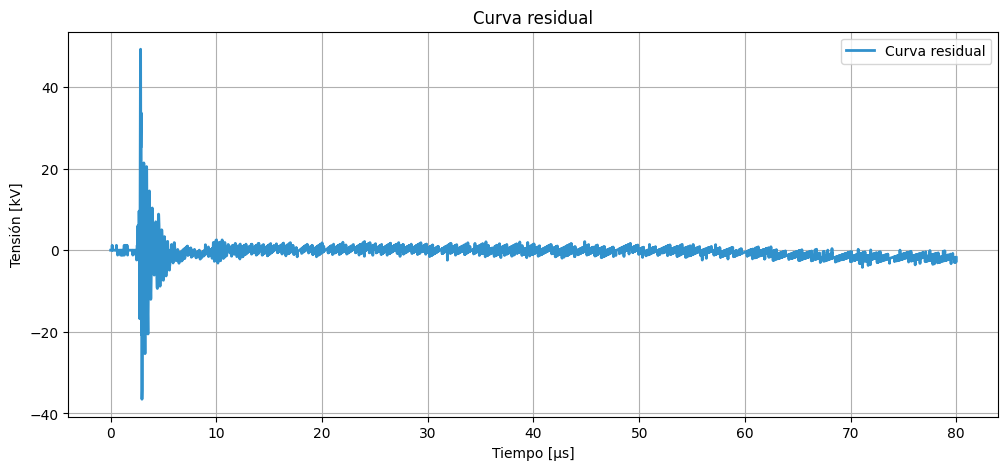
\includegraphics[width=\textwidth]{img/analisis_secuencial/LAT/5_curva_residual.png}
    \caption{Curva residual obtenida. Fuente: Propia.}
    \label{fig:curva_residual}
\end{figure}
\vspace{3\baselineskip}

Tras aplicar el filtro digital IIR de fase cero (cuya respuesta responde a la ecuación \ref{fig:funcion_tension_ensayo}), se obtiene la curva residual filtrada $R_{f}[n]$, mostrada en la figura \ref{fig:curva_filtrada}. Este filtrado mitiga la distorsión, reduciendo significativamente la amplitud del ruido de alta frecuencia (aproximadamente en un factor de \num{10} veces) y suavizando las oscilaciones.

\vspace{3\baselineskip}
\begin{figure}[H]
    \centering
    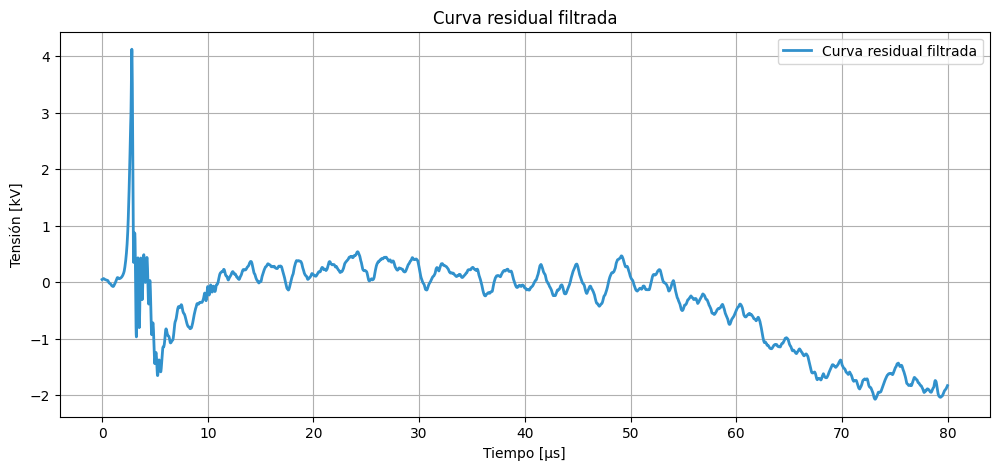
\includegraphics[width=\textwidth]{img/analisis_secuencial/LAT/6_residual_filtrada.png}
    \caption{Curva residual filtrada. Fuente: Propia.}
    \label{fig:curva_filtrada}
\end{figure}
\vspace{3\baselineskip}

La figura \ref{fig:curva_ensayo} muestra la curva de tensión de ensayo $U_\text{t}[n]$, reconstruida a partir de la suma algebraica entre la curva base y la curva residual filtrada.

\vspace{3\baselineskip}
\begin{figure}[H]
    \centering
    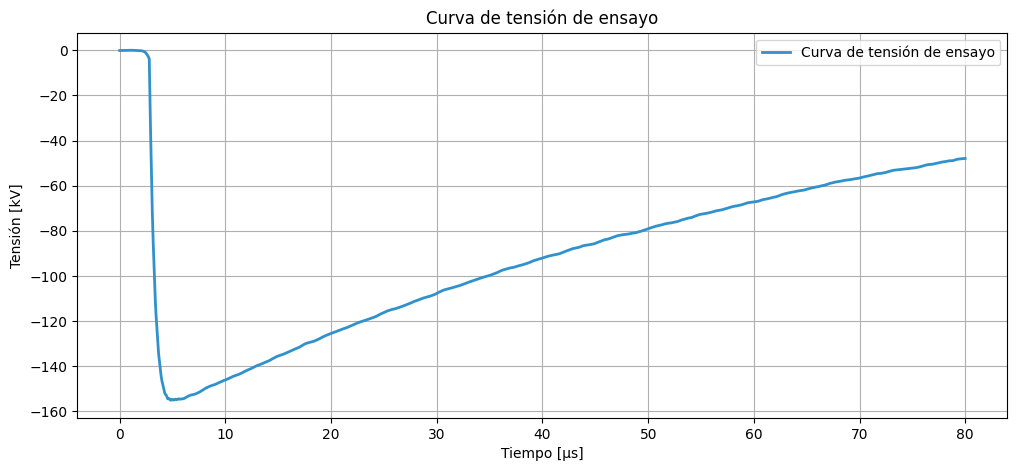
\includegraphics[width=\textwidth]{img/analisis_secuencial/LAT/7_tension_ensayo_final.png}
    \caption{Curva de tensión de ensayo $U_\text{t}[n]$. Fuente: Propia.}
    \label{fig:curva_ensayo}
\end{figure}
\vspace{3\baselineskip}

Finalmente, en la figura \ref{fig:curva_final} se superpone la curva de tensión de ensayo procesada sobre la señal original bruta. Esta comparativa evidencia la efectiva supresión del ruido de alta frecuencia y del nivel de continua, dando como resultado una forma de onda apta para la determinación precisa de sus parámetros característicos ($U_\text{t}$, $T_{1}$, $T_{2}$ y $\beta'$).

\vspace{3\baselineskip}
\begin{figure}[H]
    \centering
    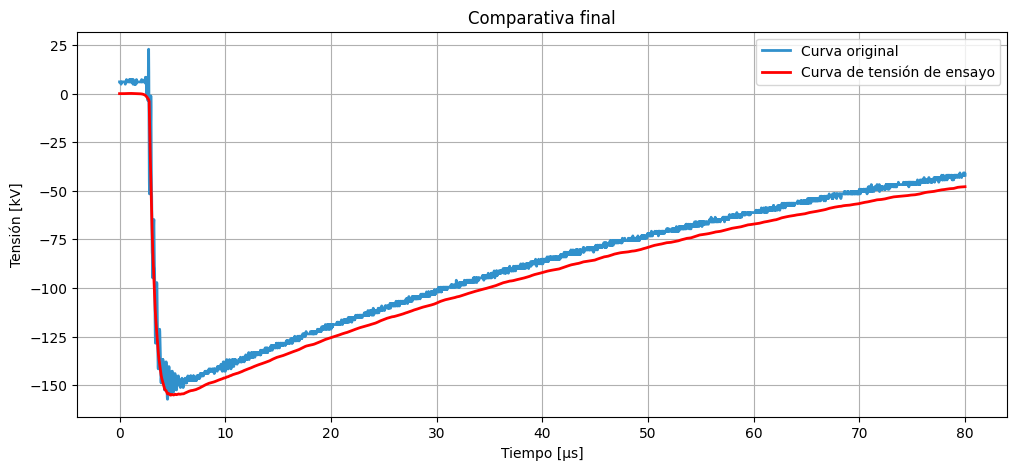
\includegraphics[width=\textwidth]{img/analisis_secuencial/LAT/8_curva_original_ensayo.png}
    \caption{Comparativa entre la curva de tensión de ensayo y la original bruta. Fuente: Propia.}
    \label{fig:curva_final}
\end{figure}
\vspace{3\baselineskip}

\section*{Ejemplo de impulso LIC}
\label{sec:ejemplo_impulso_lic}
\addcontentsline{toc}{section}{Ejemplo de impulso LIC}
\vspace{3\baselineskip}

El impulso tipo rayo cortado en la cola (LIC) analizado en esta sección corresponde a una señal sintética generada por el TDG de la norma IEC 61083-2~\cite{iec61083_2}. Este registro patrón (identificado como \texttt{LIC-M5} en el cuerpo principal del trabajo) se emplea para ilustrar el comportamiento del algoritmo de bifurcación y escalamiento paramétrico detallado en el motor de cálculo (sección \ref{subsec:motor_calculo}).

Para comprender el origen de la señal a procesar, en la figura \ref{fig:curva_original_lic} se presentan superpuestos los vectores originales proporcionados por el TDG: la onda de referencia (impulso pleno, en trazo celeste) y la onda de ensayo cortada (en trazo rojo).

\vspace{3\baselineskip}
\begin{figure}[H]
    \centering
    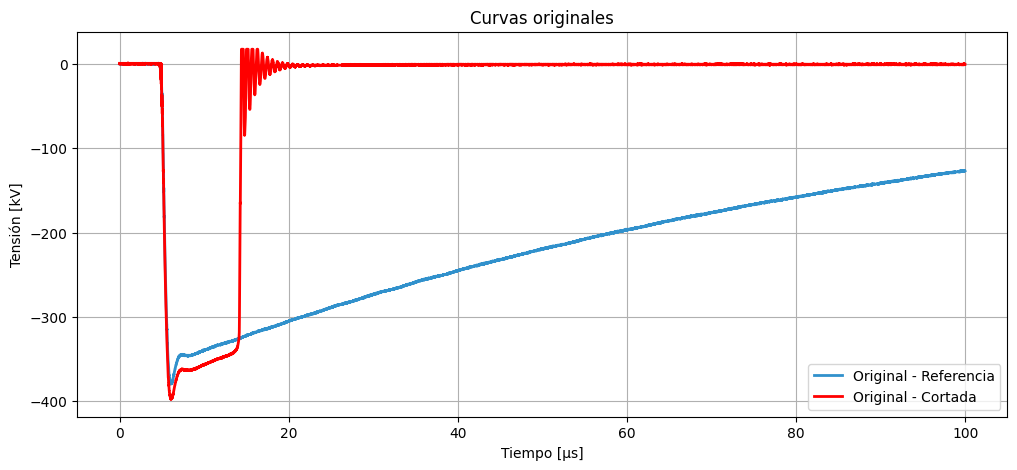
\includegraphics[width=\textwidth]{img/analisis_secuencial/LIC/0_curvas_originales.png}
    \caption{Señales originales del TDG (Referencia plena y onda cortada). Fuente: Propia.}
    \label{fig:curva_original_lic}
\end{figure}
\vspace{3\baselineskip}

A partir de este punto, el análisis se centra exclusivamente en el procesamiento de la onda cortada. La figura \ref{fig:curva_offset_lic} muestra la señal de ensayo resultante tras la evaluación y sustracción del nivel de continua $V_\text{offset}$ en el tramo de pre-disparo.

\vspace{3\baselineskip}
\begin{figure}[H]
    \centering
    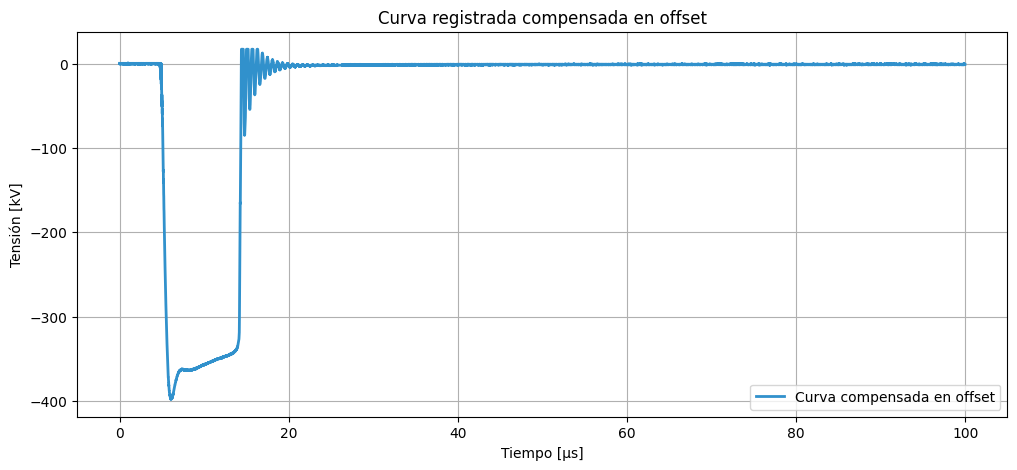
\includegraphics[width=\textwidth]{img/analisis_secuencial/LIC/1_offset_removido.png}
    \caption{Acondicionamiento de continua de la onda cortada. Fuente: Propia.}
    \label{fig:curva_offset_lic}
\end{figure}
\vspace{3\baselineskip}

En la figura \ref{fig:curva_positiva_lic} se observa la curva cortada con su amplitud y polaridad normalizadas hacia el semiplano positivo, preparándola para la fase de alineación temporal y clasificación algorítmica frente a su onda de referencia, para determinar si es una onda plena o cortada.

\vspace{3\baselineskip}
\begin{figure}[H]
    \centering
    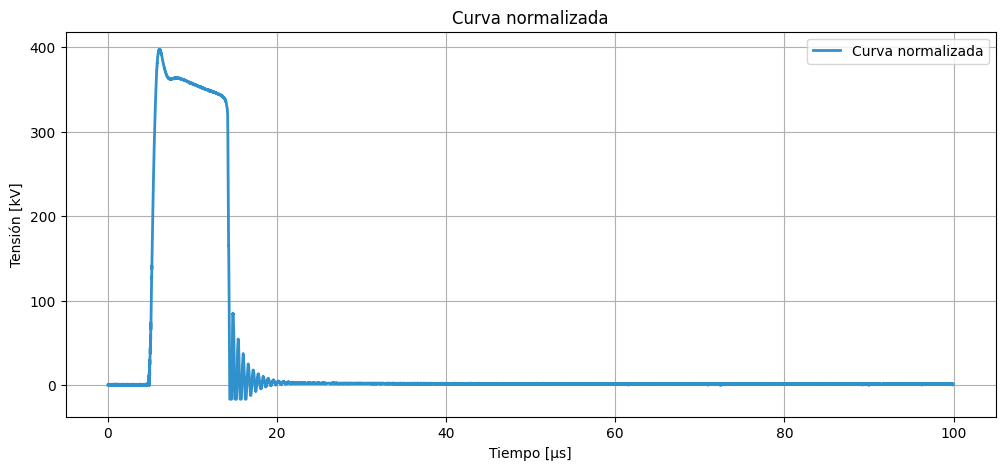
\includegraphics[width=\textwidth]{img/analisis_secuencial/LIC/2_curva_normalizada.png}
    \caption{Normalización de polaridad. Fuente: Propia.}
    \label{fig:curva_positiva_lic}
\end{figure}
\vspace{3\baselineskip}

La figura \ref{fig:curva_recortada_lic} resalta en color rojo la ventana de datos útil del frente de la onda. A diferencia del caso pleno, el algoritmo detecta la discrepancia morfológica en la cola (debida al colapso de tensión) y clasifica el impulso como LIC, por lo que utiliza este segmento resaltado únicamente para determinar el factor de escala $E$ (ecuación \ref{eq:factor_escala_e}), sin realizar un nuevo ajuste por mínimos cuadrados.

\vspace{3\baselineskip}
\begin{figure}[H]
    \centering
    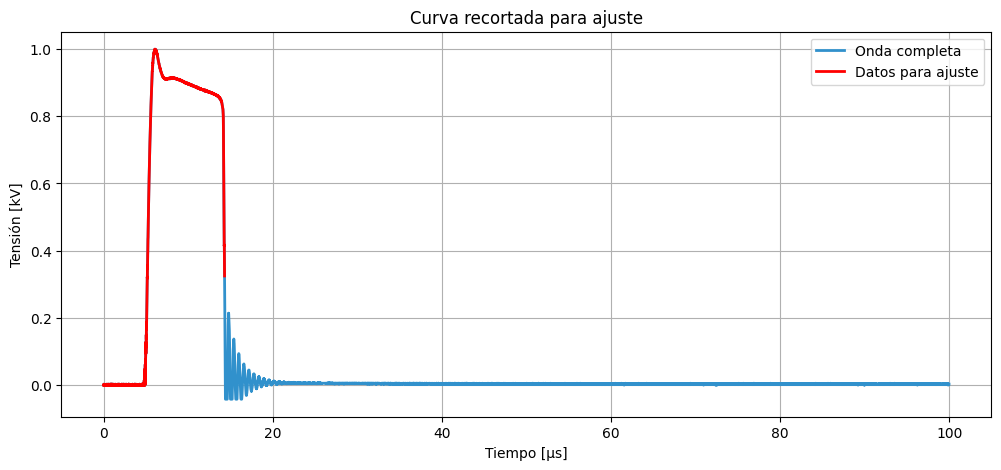
\includegraphics[width=\textwidth]{img/analisis_secuencial/LIC/3_curva_recortada.png}
    \caption{Segmentación del frente para el cálculo del factor de escala. Fuente: Propia.}
    \label{fig:curva_recortada_lic}
\end{figure}
\vspace{3\baselineskip}

En la figura \ref{fig:curva_base_lic} se observa la síntesis de la curva base de ensayo $U_\text{b}[n]$ (en trazo rojo). Esta se obtiene tomando los parámetros de la función doble exponencial de la onda plena de referencia (previamente analizada) y multiplicándolos analíticamente por el factor de escala $E$, permitiendo proyectar la trayectoria ideal que hubiera seguido la tensión de no haberse producido la descarga disruptiva.

\vspace{3\baselineskip}
\begin{figure}[H]
    \centering
    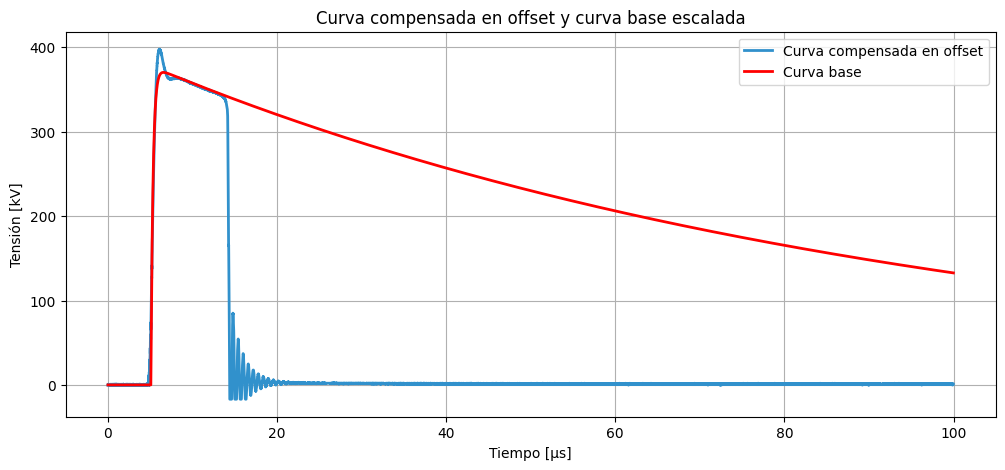
\includegraphics[width=\textwidth]{img/analisis_secuencial/LIC/4_curva_base_escalada.png}
    \caption{Sintetización de la curva base escalada analíticamente. Fuente: Propia.}
    \label{fig:curva_base_lic}
\end{figure}
\vspace{3\baselineskip}

La figura \ref{fig:curva_residual_lic} presenta la curva residual $R[n]$, resultante de restar algebraicamente la curva base idealizada de la señal compensada en \emph{offset}. Se puede observar claramente la drástica desviación negativa en el instante del corte.

\vspace{3\baselineskip}
\begin{figure}[H]
    \centering
    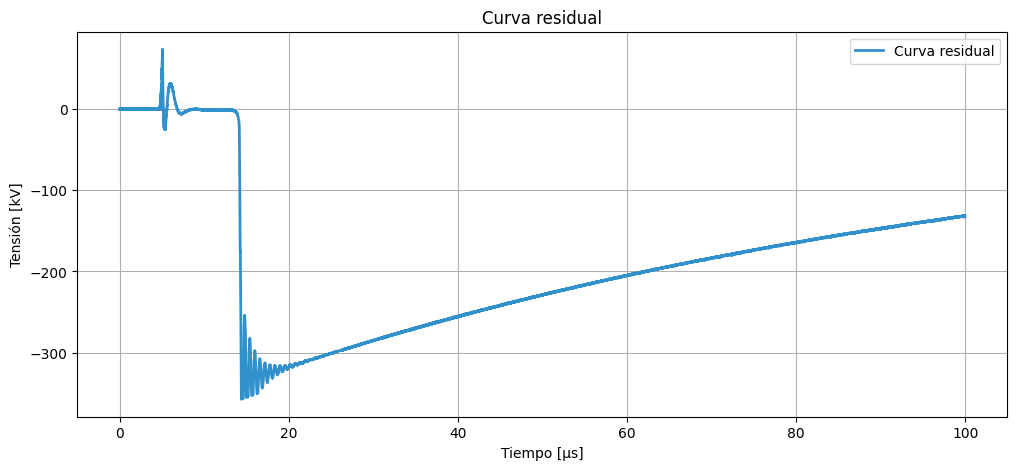
\includegraphics[width=\textwidth]{img/analisis_secuencial/LIC/5_curva_residual.png}
    \caption{Curva residual obtenida para el impulso cortado. Fuente: Propia.}
    \label{fig:curva_residual_lic}
\end{figure}
\vspace{3\baselineskip}

Al aplicar el filtro digital IIR de fase cero, se obtiene la curva residual filtrada $R_{f}[n]$ mostrada en la figura \ref{fig:curva_filtrada_lic}. El proceso de filtrado reduce las oscilaciones de alta frecuencia superpuestas en la cresta, manteniendo intacta la severidad del colapso de tensión.

\vspace{3\baselineskip}
\begin{figure}[H]
    \centering
    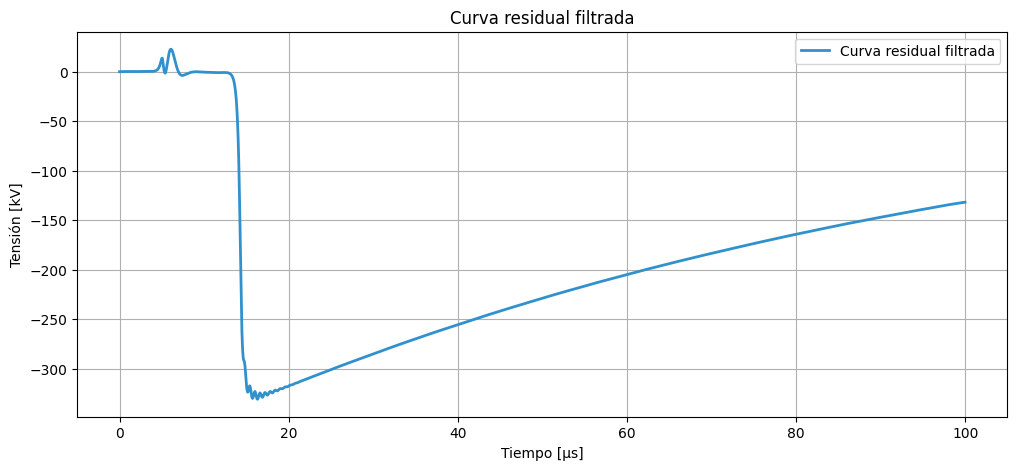
\includegraphics[width=\textwidth]{img/analisis_secuencial/LIC/6_residual_filtrada.png}
    \caption{Curva residual filtrada. Fuente: Propia.}
    \label{fig:curva_filtrada_lic}
\end{figure}
\vspace{3\baselineskip}

La figura \ref{fig:curva_ensayo_lic} muestra la curva de tensión de ensayo $U_\text{t}[n]$ final, construida mediante la adición de la curva base escalada y la curva residual filtrada.

\vspace{3\baselineskip}
\begin{figure}[H]
    \centering
    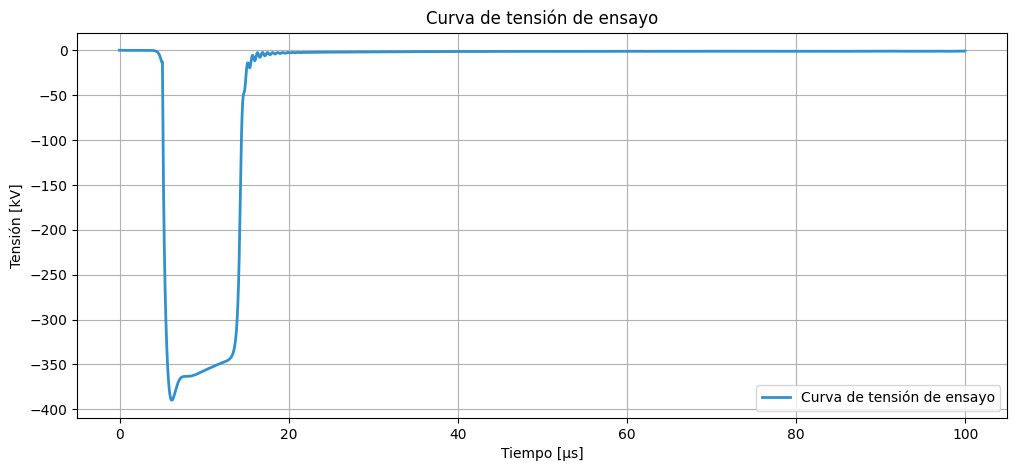
\includegraphics[width=\textwidth]{img/analisis_secuencial/LIC/7_tension_ensayo_final.png}
    \caption{Curva de tensión de ensayo $U_\text{t}[n]$. Fuente: Propia.}
    \label{fig:curva_ensayo_lic}
\end{figure}
\vspace{3\baselineskip}

Por último, en la figura \ref{fig:curva_final_lic} se superpone la curva de tensión de ensayo procesada sobre la señal original bruta del TDG. De esta curva definitiva el algoritmo extrae los parámetros normativos correspondientes al impulso cortado ($U_\text{t}$, $T_1$, $T_\text{C}$ y $\beta'$), validando la robustez del método matemático frente a colapsos abruptos.

\vspace{3\baselineskip}
\begin{figure}[H]
    \centering
    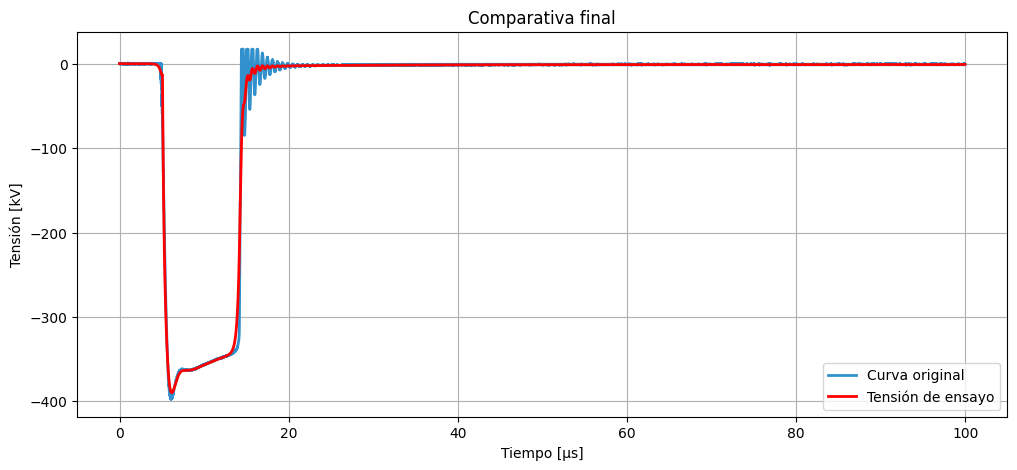
\includegraphics[width=\textwidth]{img/analisis_secuencial/LIC/8_curva_original_ensayo.png}
    \caption{Comparativa entre la curva de tensión de ensayo procesada y la original bruta. Fuente: Propia.}
    \label{fig:curva_final_lic}
\end{figure}
\vspace{3\baselineskip}